
\documentclass[a4paper, 12pt]{article}
\usepackage{geometry}
\geometry{margin=2cm}
\usepackage{graphicx} % Required for the inclusion of images
\usepackage[utf8]{inputenc}
%\usepackage{natbib} % Required to change bibliography style to APA
\usepackage{amsmath} % Required for some math elements 
\usepackage[spanish]{babel} 
%\usepackage{fontspec}
\usepackage{lineno,hyperref}
\usepackage{upgreek}
\usepackage{gensymb}
\usepackage{textcomp}
\usepackage{amssymb}
\usepackage{textgreek}
\usepackage{float}
\usepackage{fancyhdr}
\usepackage{dirtytalk}

\allowdisplaybreaks
%\textwidth18cm
%\textheight22cm
%\topmargin0cm
%\oddsidemargin2cm
%\hypersetup{hidelinks}

\usepackage{multirow}

\hypersetup{
    colorlinks=true,
    linkcolor=blue,
    }
\graphicspath{{img}}
\setlength\parindent{0pt} % Removes all indentation from paragraphs

\renewcommand{\labelenumi}{\alph{enumi}.} % Make numbering in the enumerate environment by letter rather than number (e.g. section 6)

\renewcommand{\b}{\textbf}

\newsavebox{\mygraphic}
\sbox{\mygraphic}{
\includegraphics[height=1cm]{logoUNRN.jpg}}


\pagestyle{fancy}

\fancyhead{}

\headheight 16pt

\fancyhead[LO]{\setlength{\unitlength}{1in}
	\begin{picture}(0,0)
		\put(0,0){\usebox{\mygraphic}}
	\end{picture}
	\hspace{1cm}
}

\fancyhead[CO] {\hspace{1.5cm} \large Física I: Ingenierías Ambiental, Electrónica y Telecomunicaciones}

%esto me pareció piola para enumerar los ejercicios
%lo saqué de acá: https://tex.stackexchange.com/questions/302948/numbered-exercises-as-sections
%%%%%%%%%%%%%%%%%%%%%%%%%%%%%%%%%%%%%%%%%5
\newcounter{eje}
\setcounter{eje}{0}
\newcounter{subeje}
\setcounter{subeje}{-1}
\renewcommand\thesubeje{\arabic{eje}\alph{subeje}}%
\newcommand \eje{%
  \vspace{.2cm}
  \par\noindent
  \ifnum\value{subeje}>-1
    \refstepcounter{subeje}%
    \llap{\thesubeje)\quad}%
  \else
    \refstepcounter{eje}%
    \llap{\theeje)\quad}%
  \fi
}
\begin{document}
\pagestyle{fancy}

\begin{center}

	{\Large \textbf{Parcial integrador}}
 
\vspace{.2cm}

{fecha a definir}
\end{center}

Tome para el valor de g = 9.8 m/s$^2$.

\eje{\bf TEMA 1: CINEMÁTICA}  Un piloto desea que su aeronave vuele en dirección norte respecto del suelo, pero hay viento de 60.0 km/hr que sopla de oeste a este (izquierda a derecha).

a) Si la velocidad del avión con respecto al viento es de 320.0 km/hr, ¿hacia dónde debe dirigir la aeronave, el piloto, para lograr ir hacia el norte?

b) ¿Cuál es la velocidad del avión respecto del suelo?

c) Muestre en un gráfico los vectores velocidad involucrados en la resolución del problema.

\eje{\bf TEMA 2: DINÁMICA DE UNA PARTÍCULA} El bloque con forma de cuña de la figura adjunta se acelera de tal manera que el carrito sobre este, no desliza por la pendiente, es decir que no lo hace ni para arriba, ni para abajo. Despreciando el rozamiento entre el carrito y el bloque, encuentre la aceleración de la cuña para que esto ocurra

\begin{figure}[H]
\begin{center}
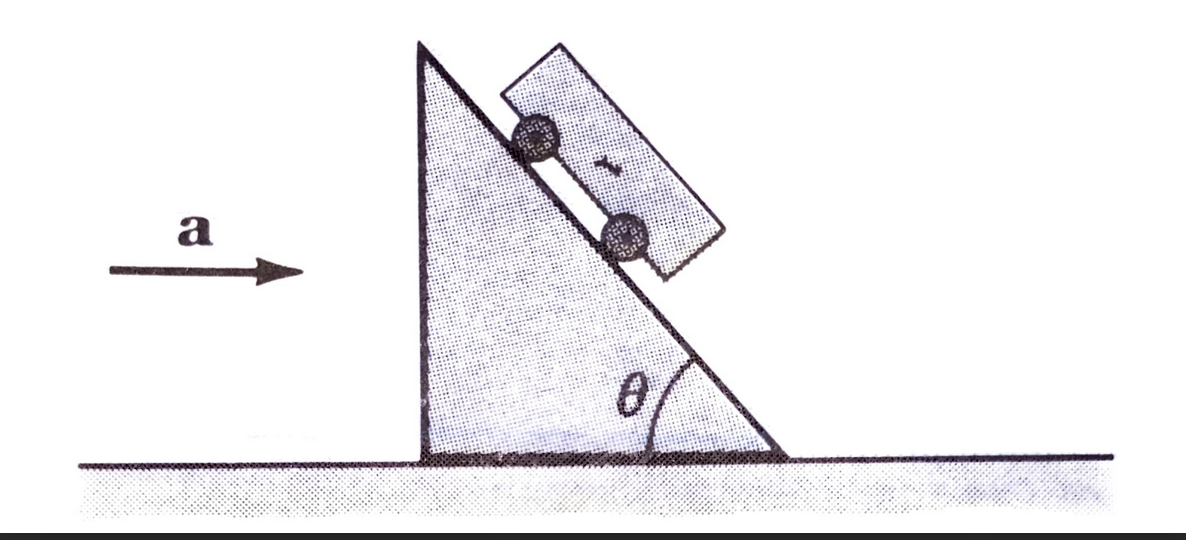
\includegraphics[clip,width = .45\columnwidth]{img/integrador2023-0.png}
\end{center}
\end{figure}

\eje{\bf TEMA 5: DINÁMICA DE UN CUERPO RÍGIDO} [EJERCICIO 16 PRÁCTICA 5] Un cilindro sube por el plano inclinado por la acción de un par de fuerzas (es decir, fuerzas iguales y opuestas) que generan un torque M, como indica la figura. 

a) Realizar el diagrama de cuerpo libre del cilindro COMPLETO. Todas las fuerzas y todos los torques (respecto del CM).

b) Hallar el valor máximo que puede tener el par de fuerzas aplicado para que el cilindro suba por el plano rodando sin deslizar. 

c) Hallar la aceleración del centro de masa del cilindro para que éste suba por el plano rodando sin deslizar 

\begin{figure}[H]
\begin{center}
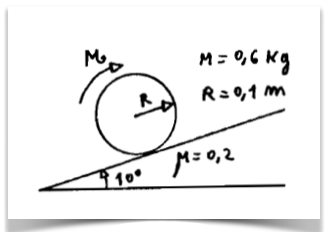
\includegraphics[clip,width = .35\columnwidth]{img/2doparcial2023-0.png}
\end{center}
\end{figure}

\end{document}